% three snapshots of the service graph, run ds_06 (values from graph_builder.py)
% thin = normal, dashed = predicted risk >= 0.5, very thick = livelock (C1-C4 hold)
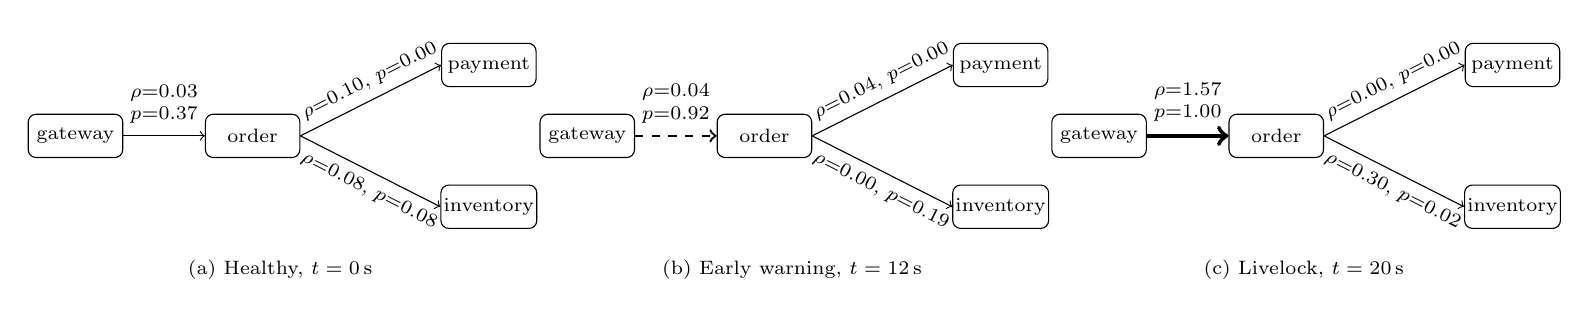
\begin{tikzpicture}[font=\scriptsize,
  svc/.style={draw, rounded corners=1mm, minimum width=12mm, minimum height=5.5mm, inner sep=1pt, font=\scriptsize},
  normal/.style={->, thin},
  warn/.style={->, thick, dashed},
  lock/.style={->, line width=1.6pt}]
\foreach \dx/\cap/\sa/\sb/\sc/\la/\lb/\lc in {
  0/{(a) Healthy, $t=0$\,s}/normal/normal/normal/{$\rho$=0.03\\$p$=0.37}/{$\rho$=0.10, $p$=0.00}/{$\rho$=0.08, $p$=0.08},
  6.5/{(b) Early warning, $t=12$\,s}/warn/normal/normal/{$\rho$=0.04\\$p$=0.92}/{$\rho$=0.04, $p$=0.00}/{$\rho$=0.00, $p$=0.19},
  13.0/{(c) Livelock, $t=20$\,s}/lock/normal/normal/{$\rho$=1.57\\$p$=1.00}/{$\rho$=0.00, $p$=0.00}/{$\rho$=0.30, $p$=0.02}} {
  \begin{scope}[xshift=\dx cm]
    \node[svc] (g) at (0,0) {gateway};
    \node[svc] (o) at (2.25,0) {order};
    \node[svc] (p) at (5.25,0.9) {payment};
    \node[svc] (i) at (5.25,-0.9) {inventory};
    \draw[\sa] (g) -- node[above=1pt, font=\scriptsize, align=center] {\la} (o);
    \draw[\sb] (o.east) -- node[above, pos=0.55, font=\scriptsize, sloped] {\lb} (p.west);
    \draw[\sc] (o.east) -- node[below, pos=0.55, font=\scriptsize, sloped] {\lc} (i.west);
    \node at (2.6,-1.7) {\cap};
  \end{scope}
}
\end{tikzpicture}
